\chapter{THIẾT KẾ PCB HOÀN CHỈNH MẠCH ĐƯỢC GIAO} 
\section{Quá trình thiết kế PCB}
\textbf{Chuyển tất cả linh kiện từ Schematic qua PCB}
\begin{figure}[H]
    \centering
    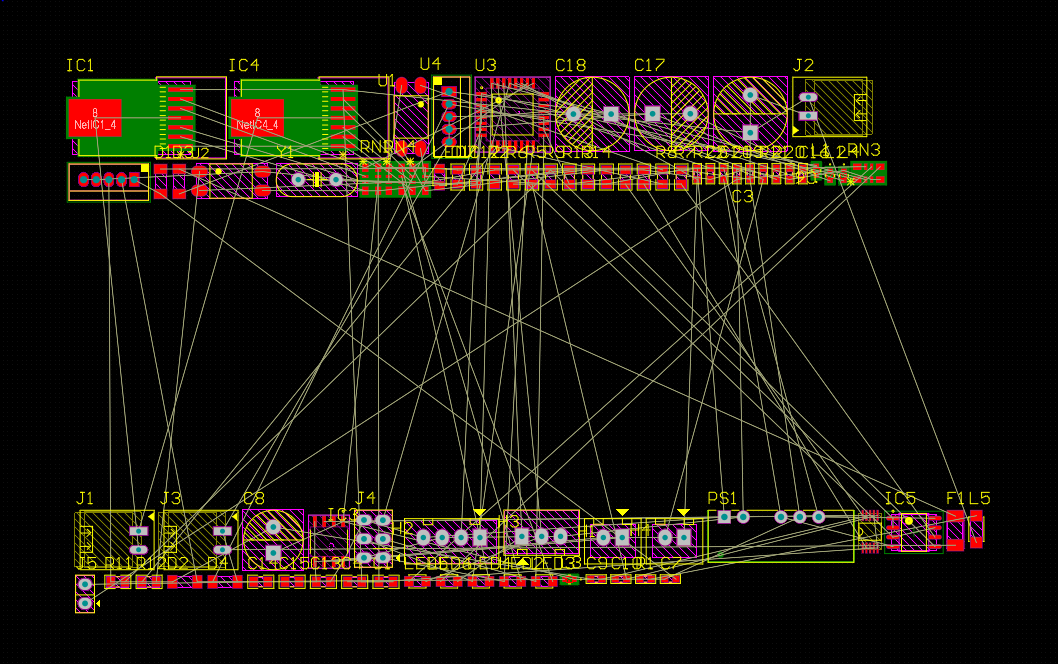
\includegraphics[width=1\textwidth]{pictures/7a.png}
\end{figure}
\begin{figure}[H]
    \centering
    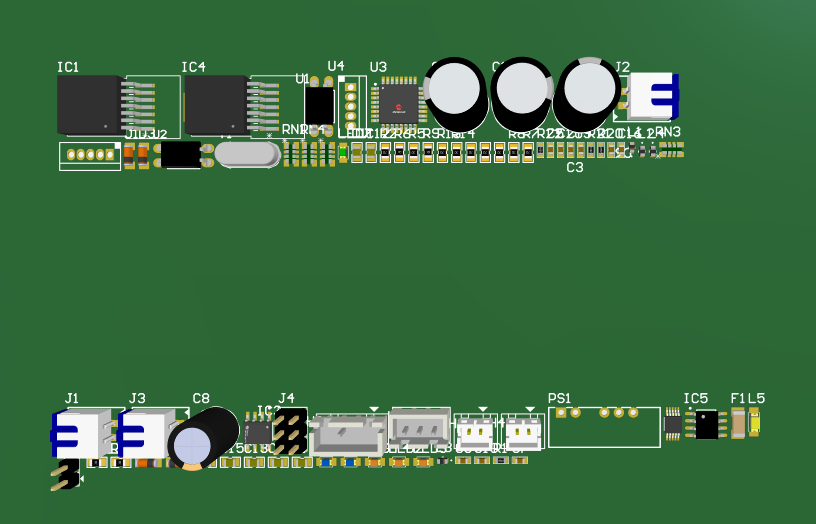
\includegraphics[width=1\textwidth]{pictures/7b.png}
\end{figure}
Ở bước này cần kiểm tra nếu có linh kiện nào không chuyển được qua PCB hay gặp các lỗi thiếu footprint như bên dưới thì cần kiểm tra lại Schematic.
\begin{figure}[H]
    \centering
    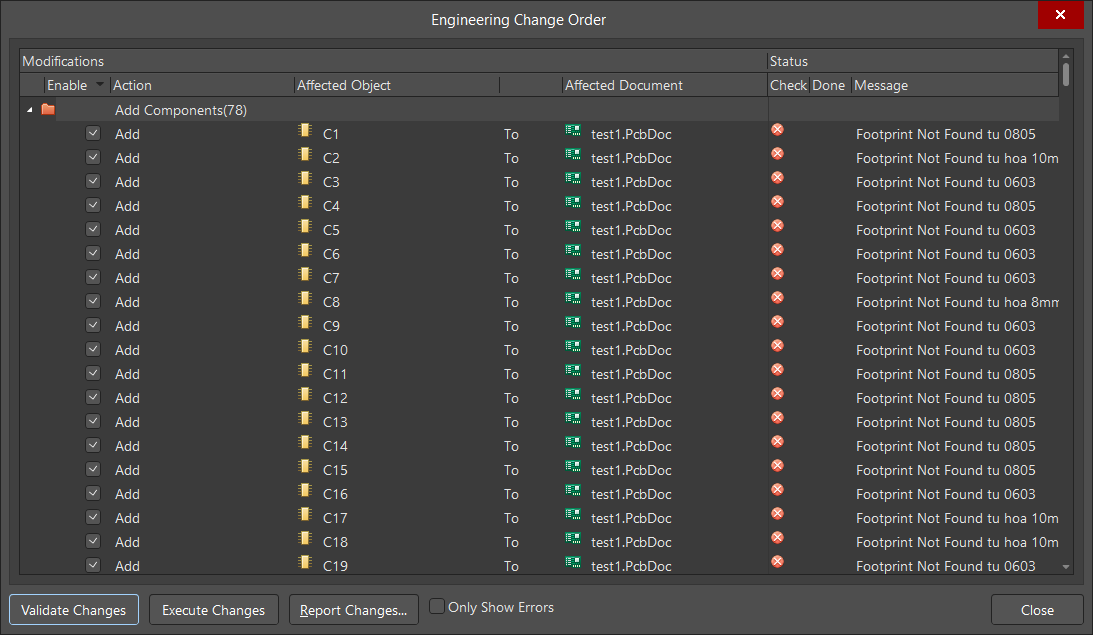
\includegraphics[width=1\textwidth]{pictures/7c.png}
\end{figure}
\cleardoublepage
\textbf{Sắp xếp vị trí linh kiện}
\begin{figure}[H]
    \centering
    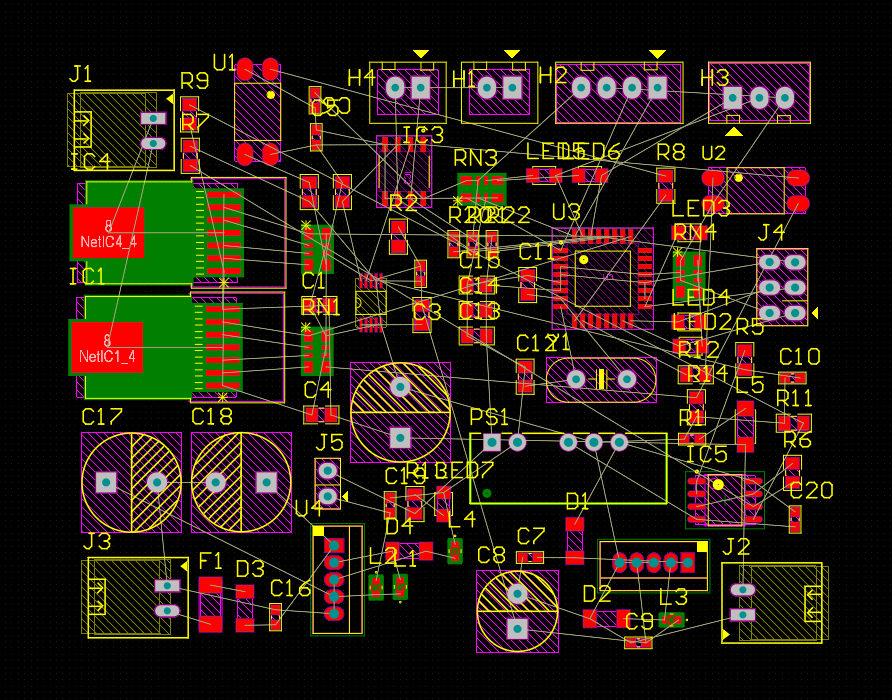
\includegraphics[width=0.8\textwidth]{pictures/7d.png}
\end{figure}
\begin{figure}[H]
    \centering
    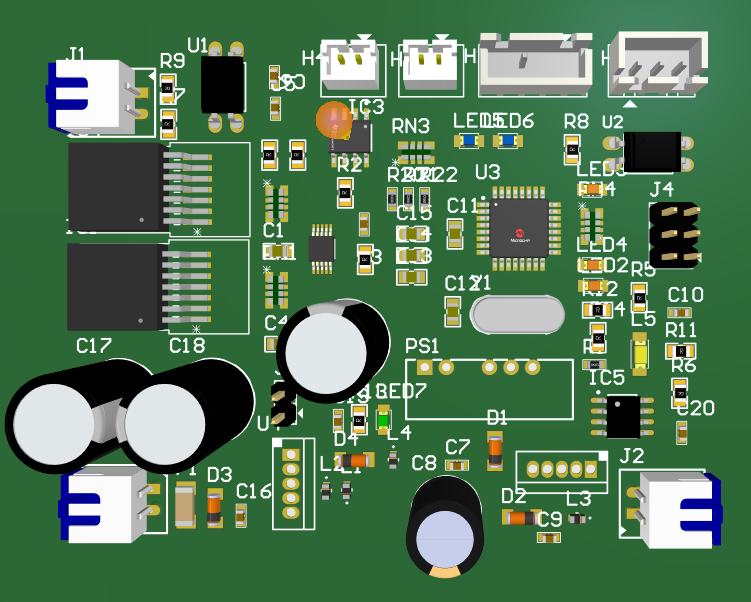
\includegraphics[width=0.8\textwidth]{pictures/7e.png}
\end{figure}
\cleardoublepage
Khi sắp xếp vị trí linh kiện cần lưu ý:
\begin{itemize}
    \item Xắp xếp để đường đi dây trên toàn mạch là ngắn nhất.
    \item Các loại linh kiện nên đồng bộ với nhau (Ví dụ trong mạch dưới đây là sử các loại linh kiện dán SMD 0805)
    \item Các terminal nên bố trí ngoài rìa. 
    \item Nên xếp theo cụm chức năng.
    \item Ngoài ra cần lưu ý khoảng cách giữa các linh kiện để không bị trùng lên nhau hoặc tồn tại quá nhiều khoảng trống không cần thiết.
\end{itemize}   
\textbf{Đi dây cho mạch}
\begin{figure}[H]
    \centering
    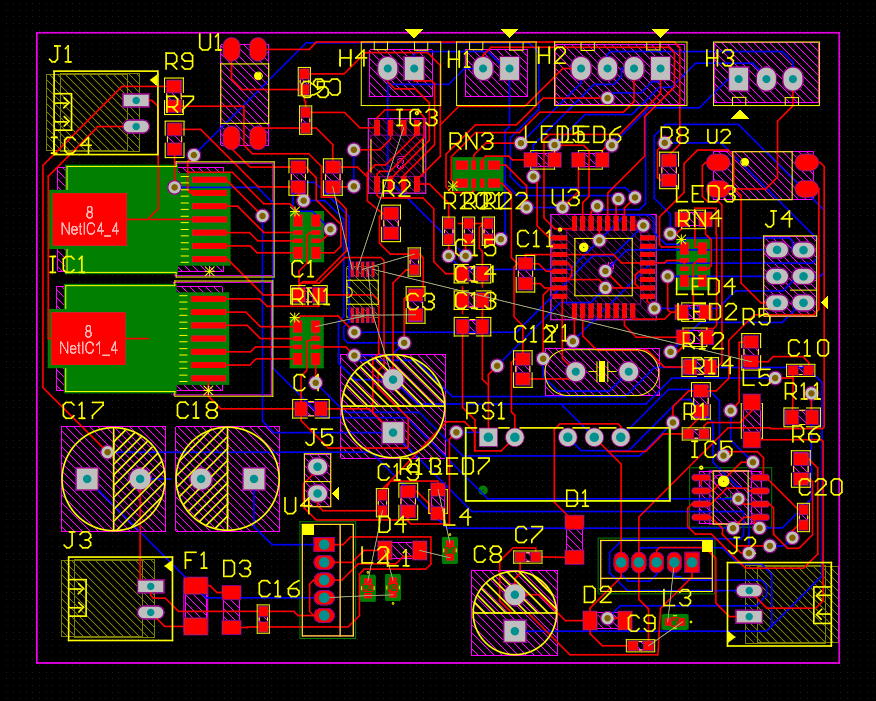
\includegraphics[width=0.8\textwidth]{pictures/7f.png}
\end{figure}
Khi đi dây cho mạch cần lưu ý kiểm tra xem có dây nào còn sót không và có dây nào không có tín hiệu không bằng chức năng Design Rule Check.
\begin{figure}[H]
    \centering
    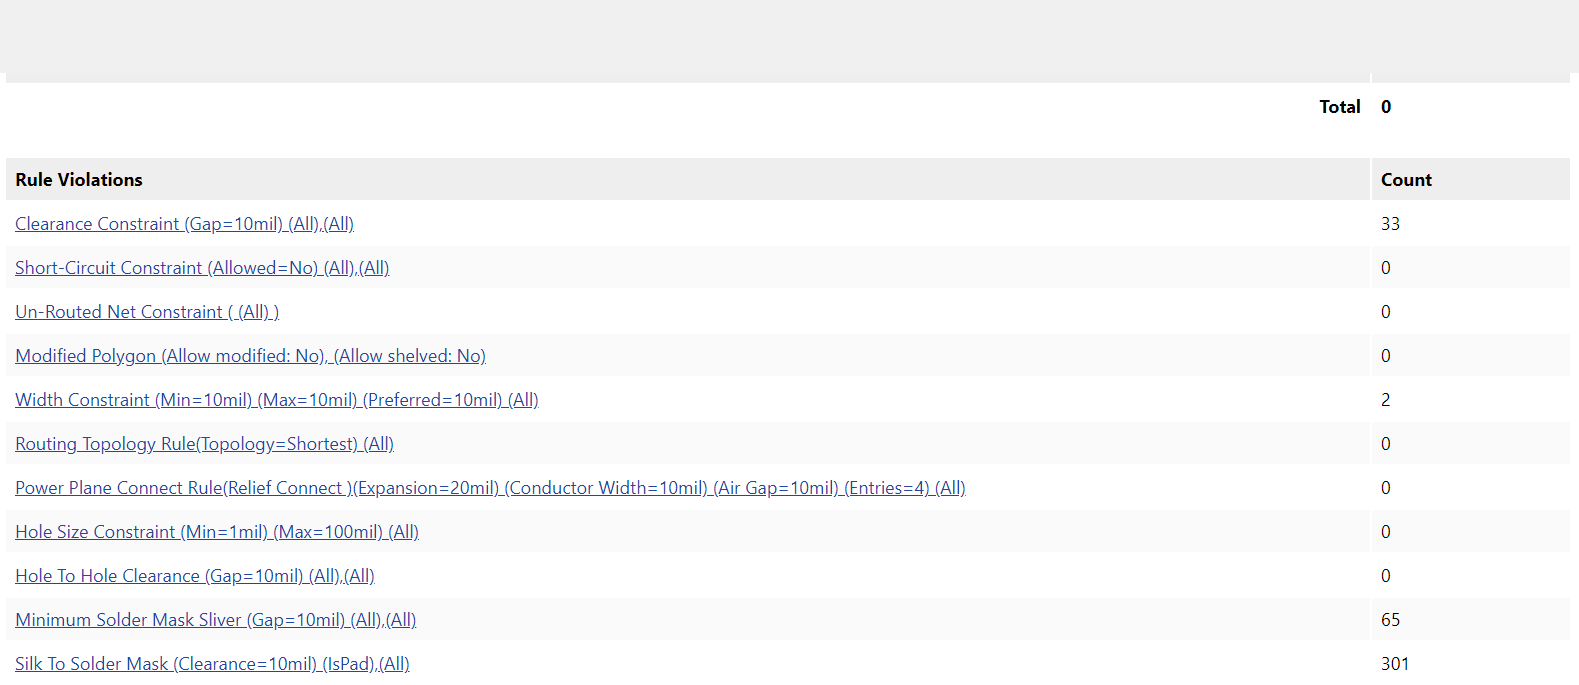
\includegraphics[width=0.8\textwidth]{pictures/7g.png}
\end{figure}
Ngoài ra ở các dây nguồn cần đi dây có độ rộng lớn hơn để tăng khả năng chịu tải và chịu nhiệt. Chúng ta sẽ tăng bề rộng các dây như sau:
\begin{figure}[H]
    \centering
    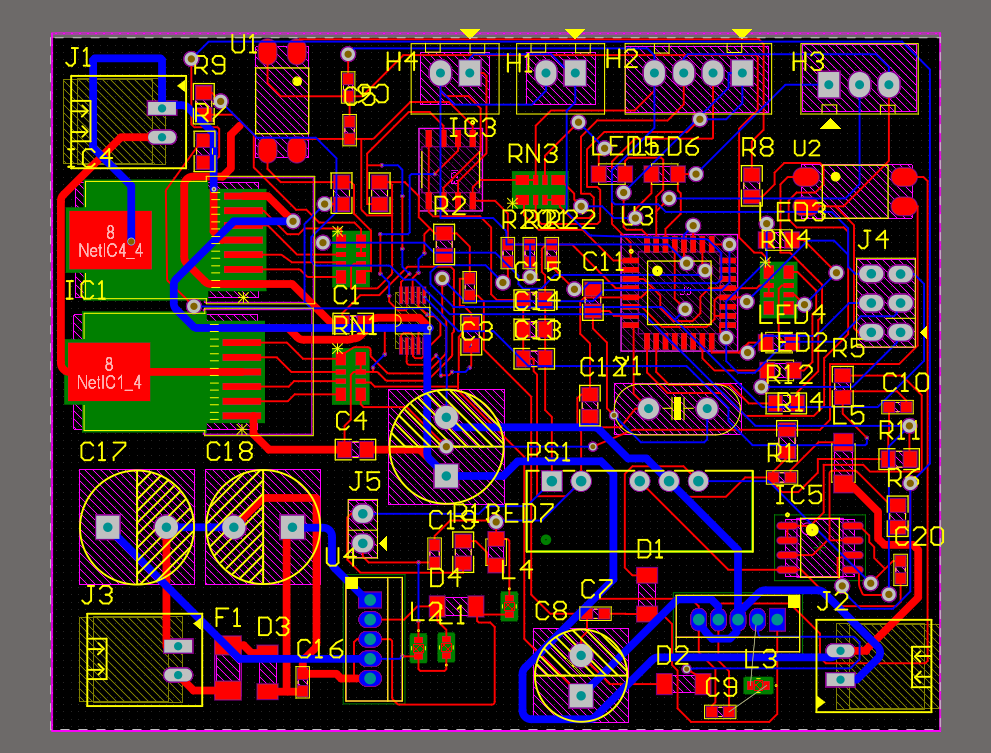
\includegraphics[width=0.8\textwidth]{pictures/7h.png}
\end{figure}
\begin{figure}[H]
    \centering
    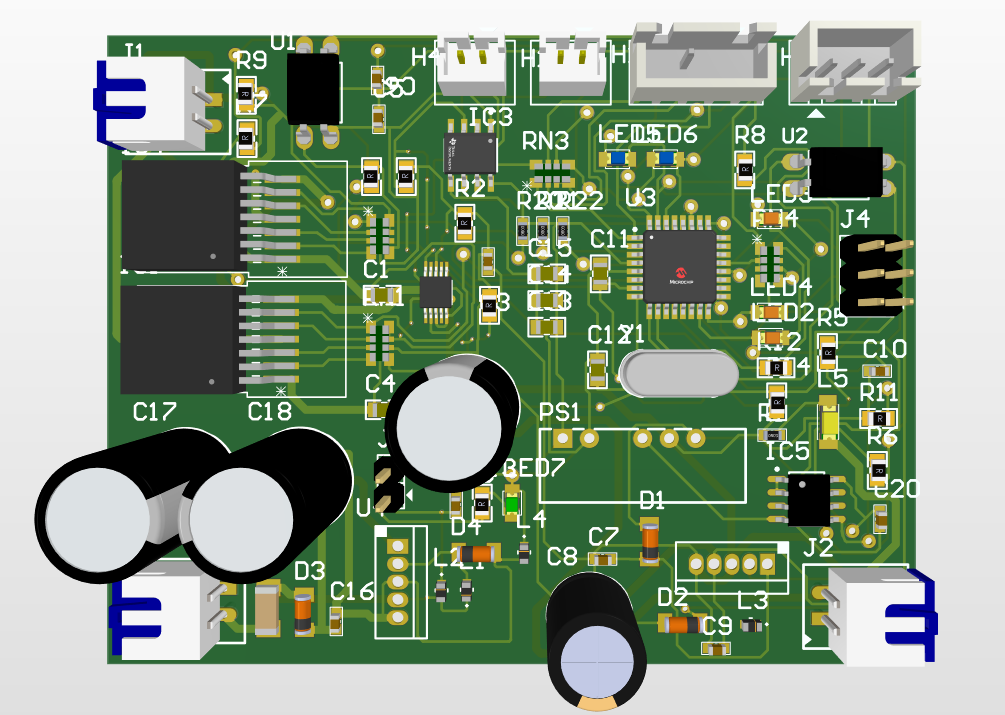
\includegraphics[width=0.8\textwidth]{pictures/7i.png}
\end{figure}
\cleardoublepage
\textbf{Phủ đồng} \\
\hspace*{0.7cm}Sau khi hoàn tất việc đi dây và sửa hết tất cả các lỗi nếu có, chúng ta thực hiện công việc cuối cùng là phủ đồng.
\begin{figure}[H]
    \centering
    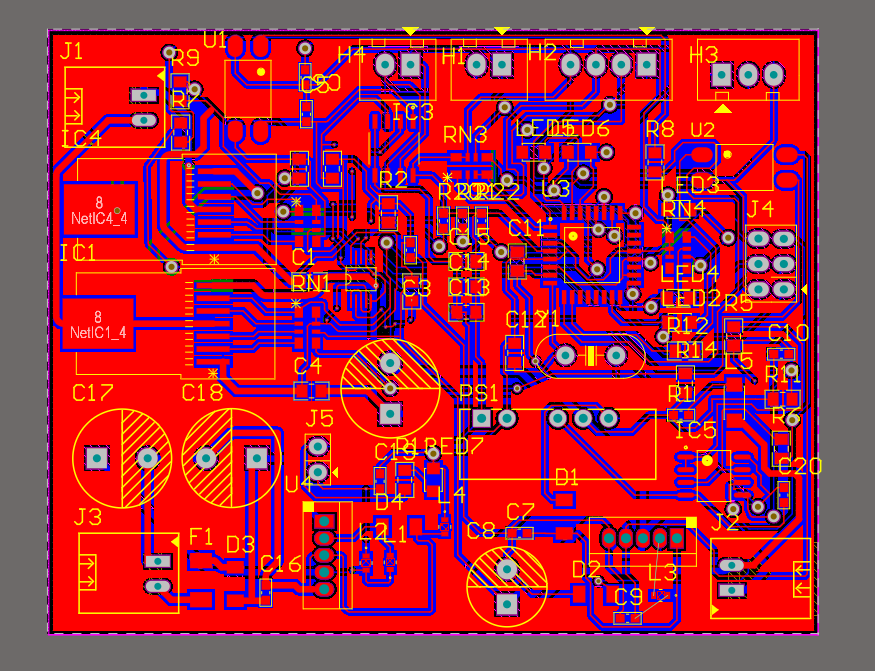
\includegraphics[width=0.8\textwidth]{pictures/7j.png}
\end{figure}
\begin{figure}[H]
    \centering
    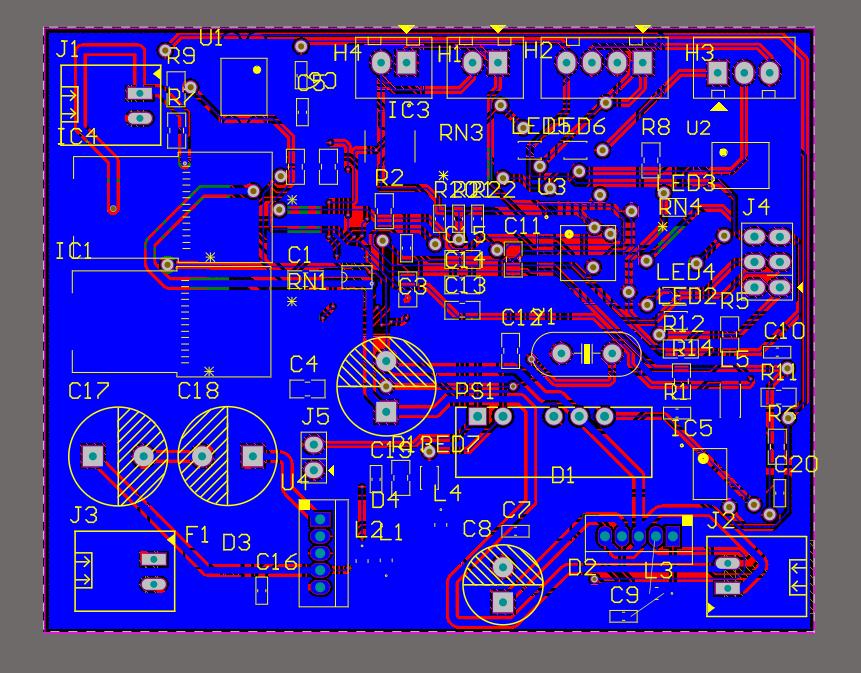
\includegraphics[width=0.8\textwidth]{pictures/7k.png}
\end{figure}
\cleardoublepage
\textbf{Hoàn thiện mạch PCB được giao}
\begin{figure}[H]
    \centering
    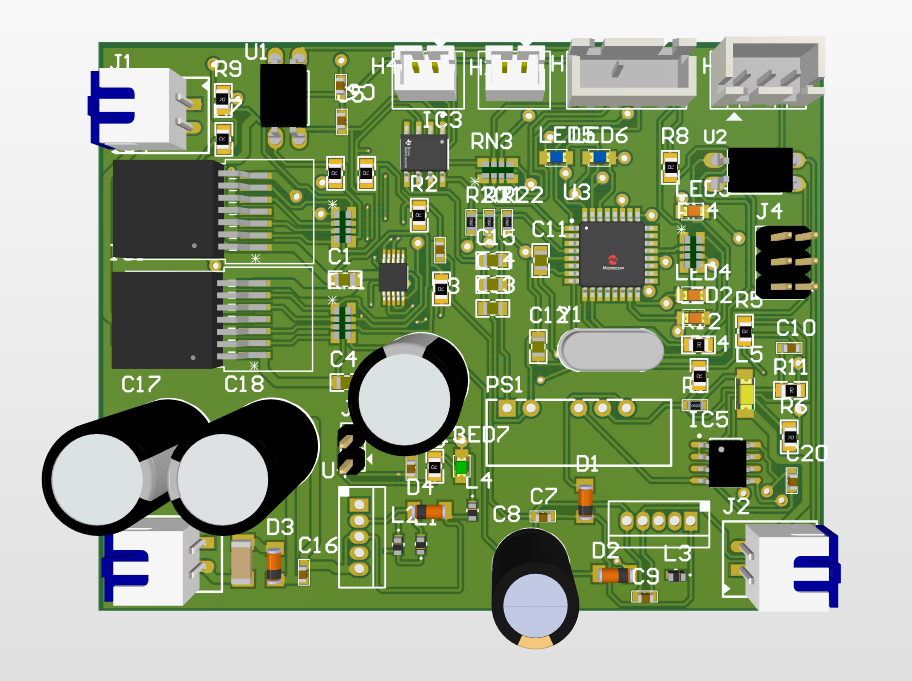
\includegraphics[width=0.9\textwidth]{pictures/7l.png}
\end{figure}
\begin{figure}[H]
    \centering
    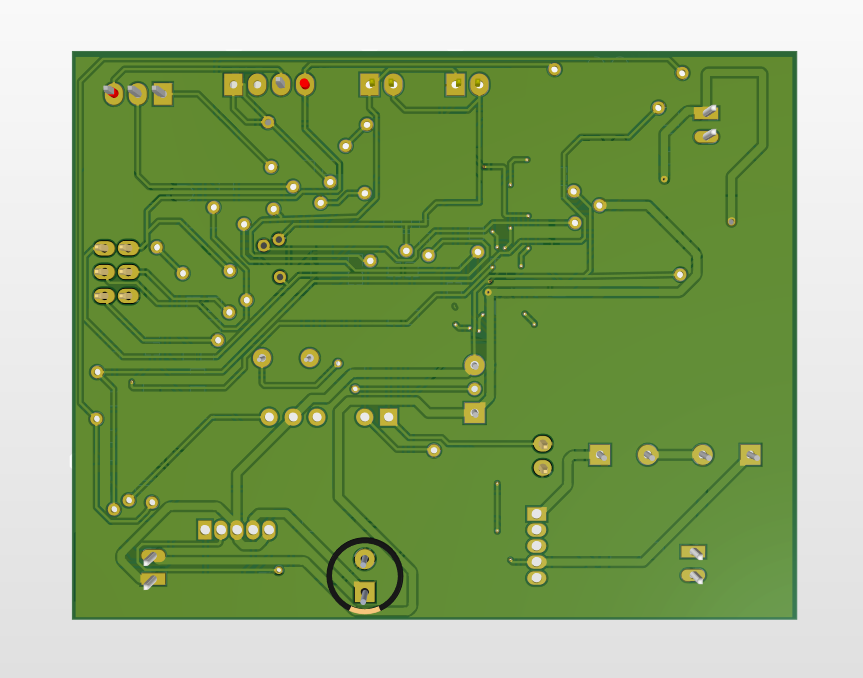
\includegraphics[width=0.9\textwidth]{pictures/7m.png}
\end{figure}
